\documentclass[11pt,a4paper]{article}
\usepackage[spanish,es-nodecimaldot]{babel}	% Utilizar español
\usepackage[utf8]{inputenc}					% Caracteres UTF-8
\usepackage{graphicx}						% Imagenes
\usepackage[hidelinks]{hyperref}			% Poner enlaces sin marcarlos en rojo
\usepackage{fancyhdr}						% Modificar encabezados y pies de pagina
\usepackage{float}							% Insertar figuras
\usepackage[textwidth=390pt]{geometry}		% Anchura de la pagina
\usepackage[nottoc]{tocbibind}				% Referencias (no incluir num pagina indice en Indice)
\usepackage{enumitem}						% Permitir enumerate con distintos simbolos
\usepackage[T1]{fontenc}					% Usar textsc en sections
\usepackage{amsmath}						% Símbolos matemáticos
\usepackage{subcaption}

% Comando para poner el nombre de la asignatura
\newcommand{\asignatura}{Simulación de Sistemas}
\newcommand{\autor}{Vladislav Nikolov Vasilev}
\newcommand{\titulo}{Práctica 4}
\newcommand{\subtitulo}{Modelos de Simulación Dinámicos Contínuos}

% Configuracion de encabezados y pies de pagina
\pagestyle{fancy}
\lhead{\autor{}}
\rhead{\asignatura{}}
\lfoot{Grado en Ingeniería Informática}
\cfoot{}
\rfoot{\thepage}
\renewcommand{\headrulewidth}{0.4pt}		% Linea cabeza de pagina
\renewcommand{\footrulewidth}{0.4pt}		% Linea pie de pagina

\begin{document}
\pagenumbering{gobble}

% Pagina de titulo
\begin{titlepage}

\begin{minipage}{\textwidth}

\centering


\includegraphics[scale=0.5]{img/ugr.png}\\

\textsc{\Large \asignatura{}\\[0.2cm]}
\textsc{GRADO EN INGENIERÍA INFORMÁTICA}\\[1cm]

\noindent\rule[-1ex]{\textwidth}{1pt}\\[1.5ex]
\textsc{{\Huge \titulo\\[0.5ex]}}
\textsc{{\Large \subtitulo\\}}
\noindent\rule[-1ex]{\textwidth}{2pt}\\[3.5ex]

\end{minipage}

\vspace{0.5cm}

\begin{minipage}{\textwidth}

\centering

\textbf{Autor}\\ {\autor{}}\\[2.5ex]
\textbf{Rama}\\ {Computación y Sistemas Inteligentes}\\[2.5ex]
\vspace{0.3cm}


\includegraphics[scale=0.3]{img/etsiit.jpeg}

\vspace{0.7cm}
\textsc{Escuela Técnica Superior de Ingenierías Informática y de Telecomunicación}\\
\vspace{1cm}
\textsc{Curso 2019-2020}
\end{minipage}
\end{titlepage}

\pagenumbering{arabic}
\tableofcontents
\thispagestyle{empty}				% No usar estilo en la pagina de indice

\newpage

\setlength{\parskip}{1em}

\section{Introducción}

El objetivo de esta práctica es el estudio de un modelo dinámico discreto basado
en las ecuaciones de Lotka-Volterra. Estas ecuaciones permiten estudiar ecosistemas
con dos especies relacionadas entre sí: las \textbf{presas} y los \textbf{depredadores}.
Estas ecuaciones se pueden ver a continuación:

\begin{equation}
\begin{split}
\frac{dx}{dt} = a_{11}x - a_{12}xy \\
\frac{dy}{dt} = a_{21}xy - a_{22}y
\end{split}
\end{equation}

\noindent donde $x$ representa la población de presas e $y$ representa la población
de depredadores. El resto de parámetros, en este caso, respresentan lo siguiente:

\begin{itemize}[label=\textbullet]
	\item $a_{11}$ representa la tasa de crecimiento de las presas. En un principio vale $5$.
	\item $a_{12}$ representa una la efectividad de los depredadores a la hora de
	capturar las presas. En un principio vale $0.05$.
	\item $a_{21}$ representa el valor nutricional de las presas (a mayor valor, menos
	presas será necesario que cace un depredador para sobrevivir). En un principio
	vale $0.0004$.
	\item $a_{22}$ representa la tasa de mortalidad de los depredadores. En este caso,
	un valor más grande indica que la población decrece más, mientras que un valor más
	bajo indica que decrece en menor medida, y por tanto, los miembros de la población
	son más longevos. Inicialmente vale $0.2$.
\end{itemize}

Una vez explicado el sistema a estudiar y una vez que se ha implementado siguiendo
las instrucciones proporcionadas, vamos a experimentar con los parámetros del sistema
para ver cómo evolucionan las dos especies en función de estos. También haremos
una comparativa entre los dos métodos de integración que se proponen: el método de Euler
y el de Runge-Kutta.

Para todas las experimentaciones vamos a simular desde $\texttt{tinic} = 0$ hasta $\texttt{tfin} = 200$,
ya que para valores más altos de \texttt{tfin} no se pueden apreciar bien
los resultados en las gráficas. El intervalo de cálculo será en un principio de 0.1, pero a la hora
de comparar los distintos métodos de integración será variable. Los demás valores se van
a ir variando con el objetivo de estudiar el funcionamiento del sistema.

\section{Experimentación con las condiciones iniciales}

Lo primero que vamos a hacer es experimentar con las condiciones iniciales, con el
objetivo de ver cómo cambia el comportamiento del sistema en función de estos.

Lo primero que vamos a hacer es establecer los valores de los parámetros $a_{ij}$,
ya que estos se mantendrán fijos a lo largo de la experimentación. En este caso,
los valores son los siguientes:

$$
	a_{11} = 5, \; a_{12} = 0.05, \; a_{21} = 0.0004, \; a_{22} = 0.2
$$

En un primer instante, se pide que los valores iniciales de las dos poblaciones
sean $x = \frac{a_{22}}{a_{21}}$ e $y = \frac{a_{11}}{a_{12}}$. Si los calculamos,
obtenemos que $x = 500$ e $y = 100$. Si ahora ejecutamos el simulador con los parámetros
correspondientes, obtenemos los siguientes resultados:

\begin{figure}[H]
	\centering
	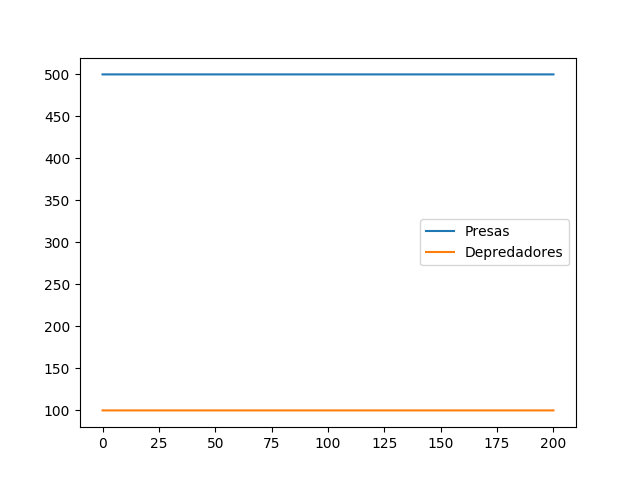
\includegraphics[scale=0.6]{img/x500y100}
	\caption{Simulación del sistema con 500 presas ($x$) y 100 depredadores ($y$).}
\end{figure}

Vemos que en este caso el sistema permanece en equilibrio, ya el número de individuos
que componen las dos poblaciones no varía a lo largo del tiempo. Esto se debe a que
los valores iniciales son proporcionales a los parámetros $a_{ij}$, de forma que
el número inicial de presas depende de la tasa de crecimiento de los depredadores
y del valor nutricional de las presas, mientras que el número inicial de depredadores
depende de la tasa de incremento de las presas y de la efectividad de los depredadores.
De esta forma, nos podemos asegurar que el número inicial de individuos sea el justo para
que en ningún momento exista una fluctuación en el número de individuos que componen las
poblaciones.

Habiendo visto la situación de equilibrio anterior, vamos a ver ahora qué es lo que pasa
cuando se modifican los valores iniciales para las dos poblaciones. Vamos a probar, por ejemplo,
con un sistema en el que hayan más presas, conservando el mismo número de depredadores.
Por ejemplo, vamos a establecer que $x = 600$, para ver qué es lo que sucede al salir de la
zona de equilibrio. Los resultados se pueden ver a continuación:

\begin{figure}[H]
\centering
\begin{subfigure}{.5\textwidth}
	\centering
	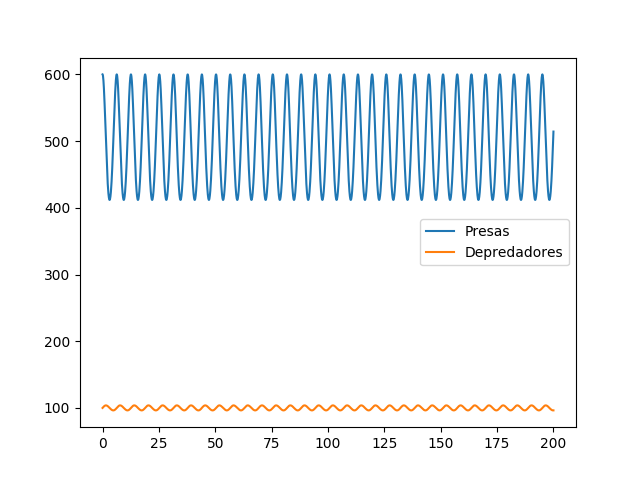
\includegraphics[scale=0.45]{img/x600y100}
	\subcaption{Evolución de las dos poblaciones en conjunto}
	\label{fig:x600}
\end{subfigure}%
\begin{subfigure}{.5\textwidth}
	\centering
	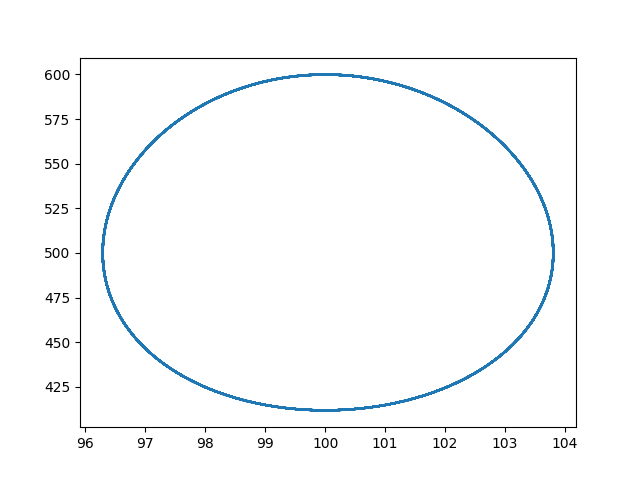
\includegraphics[scale=0.45]{img/circulo-x600}
	\subcaption{Número de presas en función del número de depredadores.}
	\label{fig:circ-x600}
\end{subfigure}
\caption{Resultados para un número inicial de 600 presas.}
\end{figure}

Tal y como vemos en la figura \ref{fig:x600}, al aumentar el número inicial de presas y hacer que
su valor no dependa de los parámetros $a_{ij}$ se empiezan a producir cambios en las dos poblaciones.
Vemos que ambas poblaciones van creciendo y dereciendo de la misma forma periódicamente. Vemos también
que estos crecimientos están acotados, ya que no se superan ciertos rangos de valores. Se puede observar
que cuando la población de presas disminuye, se produce un aumento en la población de depredadores.
Lo mismo sucede en el caso contrario: cuando decrece la de depredadores, aumenta la de presas. Estas evoluciones
son completamente lógicas y razonables, ya que a menos presas, menos comida tendrán los depredadores, y por tanto
un mayor número de ellos morirá. A más presas, más comida, y por tanto más va a crecer la población de depredadores.
La evolución de las dos poblaciones se puede ver también en la figura \ref{fig:circ-x600}, donde vemos
la evolución de la población de presas en función de la de depredadores. Vemos que la evolución tiene
forma circular, casi como una elipse. Por tanto, observando ambas gráficas, podemos concluir que con estos
valores iniciales, las dos poblaciones crecen y decrecen de forma equilibrada, sin extinguirse ninguna de ellas
en ningún momento.

Ahora, si probamos a modificar el número inicial de depredadores y hacemos que tenga el valor
$y = 150$, sin modificar el número de presas iniciales (es decir, dejando dicho número a 500),
obtenemos los siguientes resultados:

\begin{figure}[H]
\centering
\begin{subfigure}{.5\textwidth}
	\centering
	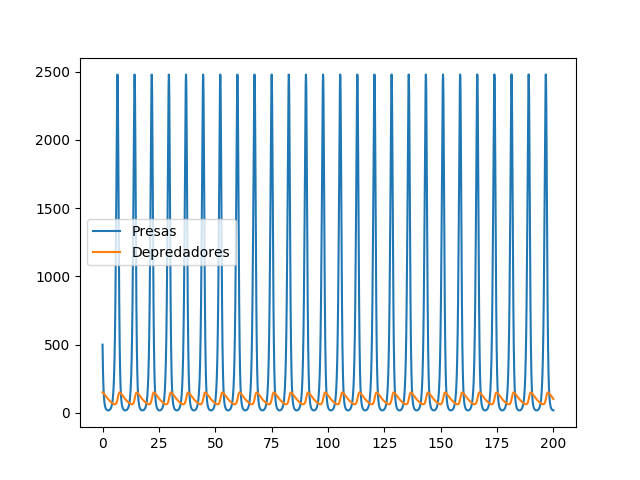
\includegraphics[scale=0.45]{img/x500y150}
	\subcaption{Evolución de las dos poblaciones en conjunto}
	\label{fig:y150}
\end{subfigure}%
\begin{subfigure}{.5\textwidth}
	\centering
	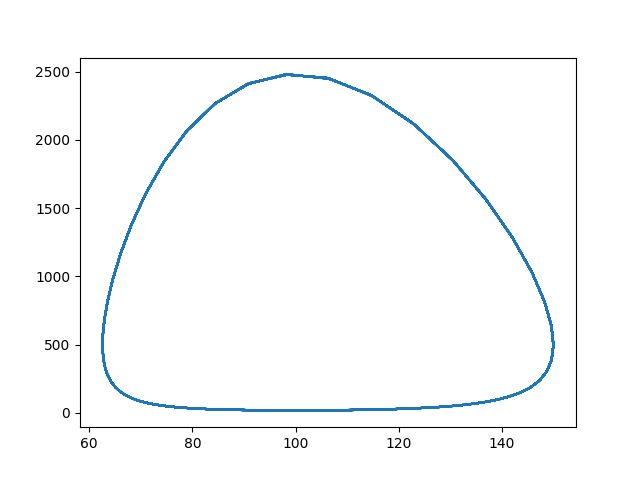
\includegraphics[scale=0.45]{img/circulo-y150}
	\subcaption{Número de presas en función del número de depredadores.}
	\label{fig:circ-y150}
\end{subfigure}
\caption{Resultados para un número inicial de 150 depredadores.}
\label{fig:dep}
\end{figure}

Vemos que en este caso sucede algo parecido al anterior, ya que no se extingue ninguna de las especies.
No obstante, la evolución de las dos poblaciones es algo diferente. Aquí podemos ver que los aumentos
y las disminuciones del número de presas es mucho más prounciado que en el caso anterior, ya que los
valores máximos alcanzados son mucho más altos que en el caso anterior. Los mínimos también son muy diferentes,
ya que se quedan bastante cerca de 0, es decir, al borde de la extinción. El crecimiento de la población
de depredadores también ha experimentado un ligero cambio, ya que ahora se alcanzan valores máximos algo
más altos. Además, la forma del crecimiento ha cambiado, ya que ha pasado de tener una forma sinusoidal a otra
que recuerda más a una ``ola''. Si ahora observamos la figura \ref{fig:circ-y150} vemos que, efectivamente, ha
habido un cambio bastante importante respecto al caso anterior. La forma ha dejado de parecerse a una elipse para
parecer una circunferencia bastante deformada. La parte de abajo está bastante aplanada, lo cuál implica
un decrecimiento muy rápido del número de depredadores una vez que el de presas es casi 0. Después, se produce
un crecimiento en el número de presas hasta llegar al máximo, y posteriormente un decrecimiento de nuevo debido
a que el número de depredadores se ha visto incrementado debido a la presencia de más comida. Por tanto, a la vista
de los resultados, vemos que en este sistema también hay una evolución equilibrada de las dos especies, sin que
ninguna de ellas se extinga.

\section{Experimentación con los parámetros}

Una vez que hemos experimentado con los valores iniciales de las dos poblaciones, vamos
a probar a modificar los parámetros $a_{ij}$ para ver qué cambios se producen en el sistema.
Para ello, vamos a partir del sistema con 600 presas y 100 depredadores, ya que es el que tiene
una evolución más balanceada de los dos que hemos probado anteriormente.

Primero, vamos a probar a modificar el parámetro $a_{11}$, el cuál recordemos que se
relaciona con la tasa de crecimiento de las presas. Vamos a probar a incrementar dicho
valor, para ver qué es lo que sucede en el sistema. Vamos a cambiar dicho valor, por ejemplo,
a 10, de forma que las presas crezcan en mayor medida. A continuación podemos ver los resultados:

\begin{figure}[H]
\centering
\begin{subfigure}{.5\textwidth}
	\centering
	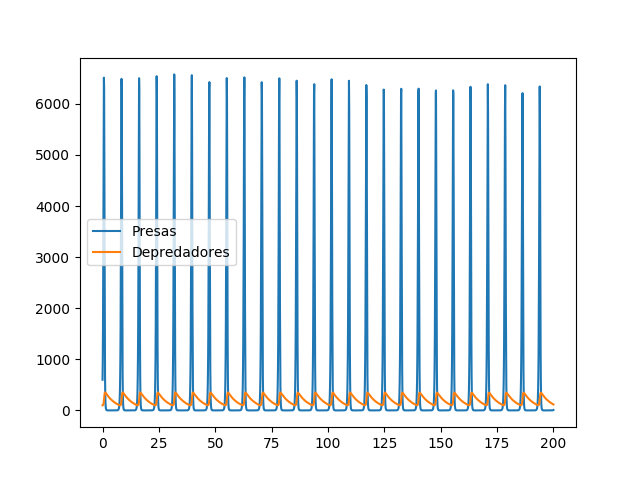
\includegraphics[scale=0.45]{img/a11-10}
	\subcaption{Evolución de las dos poblaciones en conjunto}
\end{subfigure}%
\begin{subfigure}{.5\textwidth}
	\centering
	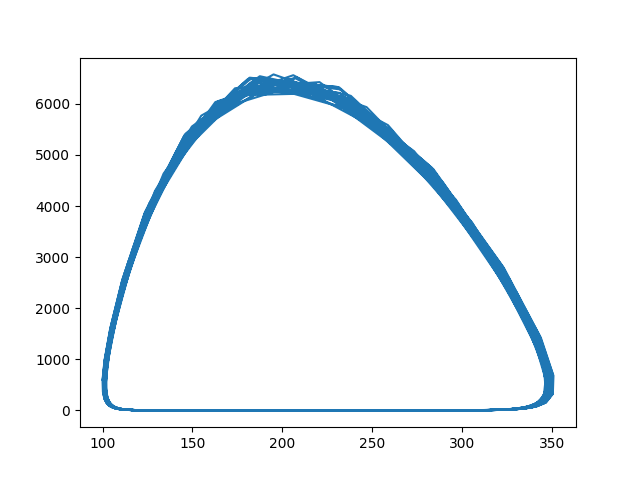
\includegraphics[scale=0.45]{img/circulo-a11}
	\subcaption{Número de presas en función del número de depredadores.}
\end{subfigure}
\caption{Resultados para $a_{11} = 10$.}
\end{figure}

En general, los resultados obtenidos se asemejan a los que se pueden ver en la figura
\ref{fig:dep}. La principal diferencia es que el máximo al que llega la población de
presas va cambiando, mientras que el de los depredadores parece mantenerse constante.
Parece que existe cierta tendencia a la baja en cuanto al número máximo de individuos
en la población de presas, a pesar del crecimiento irregular de esta. Esto se puede
ver mejor en la evolución conjunta, donde se puede ver que algunas zonas son más gruesas
debido a que los valores que se van obteniendo difieren a lo largo de la simulación.
En este segundo gráfico vemos también que la población de depredadores es capaz de crecer
hasta valores que hasta ahora no habíamos visto, debido a que hay más presas a las que
cazar, ya que se reproducen en una mayor medida, y por tanto, se generan más presas.

Ahora, si probamos a modificar el valor de $a_{12}$ a por ejemplo $0.15$ (es decir,
los depredadores son algo más eficaces) obtenemos los siguientes resultados:

\begin{figure}[H]
\centering
\begin{subfigure}{.5\textwidth}
	\centering
	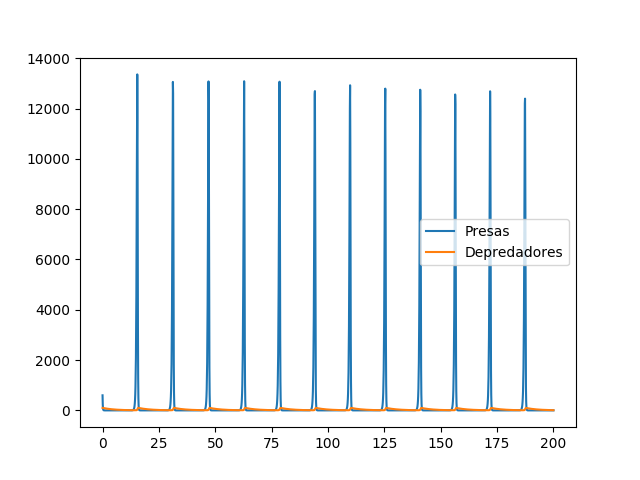
\includegraphics[scale=0.45]{img/a12}
	\subcaption{Evolución de las dos poblaciones en conjunto}
\end{subfigure}%
\begin{subfigure}{.5\textwidth}
	\centering
	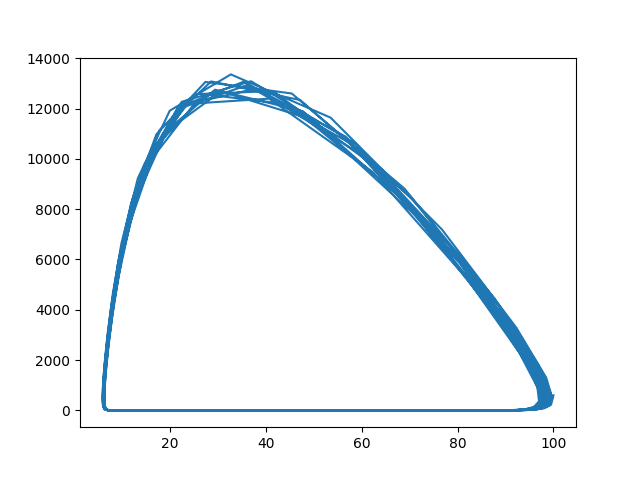
\includegraphics[scale=0.45]{img/circulo-a12}
	\subcaption{Número de presas en función del número de depredadores.}
\end{subfigure}
\caption{Resultados para $a_{12} = 0.15$.}
\end{figure}

Aquí podemos ver que si los depredadores son más efectivos se producen menos cazas,
lo cuál implica que tanto la población de las presas crezca mucho más que en los casos
anteriores como que el número de depredadores baje mucho más, hasta casi extinguirse,
ya que cuando cazan matan más presas, y por tanto se quedan con menos comida disponible,
lo cuál va a hacer que acaben muriendo por inanición.

Si probamos a hacer que las presas tengan un mayor valor nutritivo (parámetro $a_{21}$), de por ejemplo
$0.01$, obtenemos los resultados que se pueden ver en la figura \ref{fig:a21}.
Vemos que, al ser las presas más nutritivas, la población de depredadores crece muchísimo
de golpe en el momento en el que se produzca una cacería, las cuáles, al igual que en el caso
anterior, son menos comunes, pero aquí debido a otros factores, entre los cuáles encontramos
por ejemplo un mayor tiempo de recuperación de la población de presas. Este incremento se debe
a que los depredadores están mejor alimentados, con lo cuál posiblemente puedan vivir más tiempo
y reproducirse más. Como consecuencia, tal y como se dijo anteriormente, se tiene que la
población de presas tarda más tiempo en recuperarse, ya que permanece mucho tiempo al borde
de la extinción debido a la gran presencia de depredadores que hay. Una vez que el número
de depredadores baje lo suficiente debido a que hay pocas presas que cazar, entonces el
número de presas puede volver a crecer hasta unos valores que los situarían fuera del riesgo de
extinción, próximos a los iniciales. Una vez que se lleguen a esos valores, se volvería a repetir
todo el proceso.

Por último, podemos probar a modificar el valor del parámetro $a_{22}$, el cuál se relaciona
con la tasa de mortalidad de los depredadores. Vamos a probar a subir el valor hasta
$0.5$, para ver cómo son afectadas las dos poblaciones por dicho parámetro. Los resultados
se pueden ver en la figura \ref{fig:a22}.

\begin{figure}[H]
\centering
\begin{subfigure}{.5\textwidth}
	\centering
	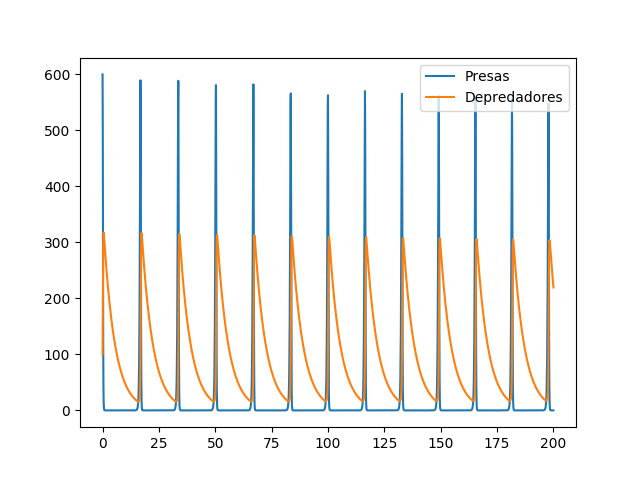
\includegraphics[scale=0.45]{img/a21}
	\subcaption{Evolución de las dos poblaciones en conjunto}
\end{subfigure}%
\begin{subfigure}{.5\textwidth}
	\centering
	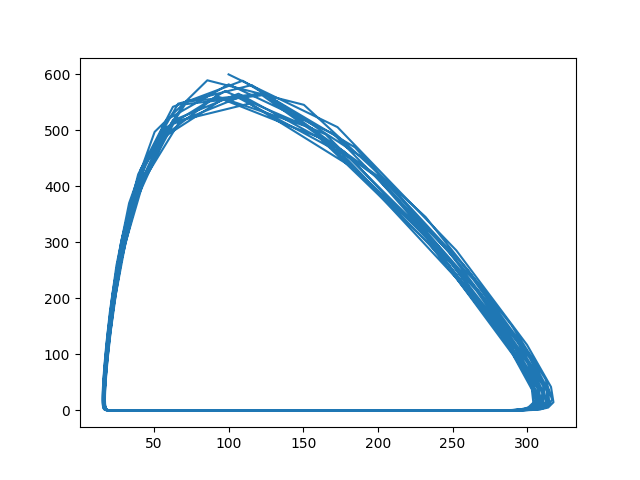
\includegraphics[scale=0.45]{img/circulo-a21}
	\subcaption{Número de presas en función del número de depredadores.}
\end{subfigure}
\caption{Resultados para $a_{21} = 0.01$.}
\label{fig:a21}
\end{figure}

\begin{figure}[H]
\centering
\begin{subfigure}{.5\textwidth}
	\centering
	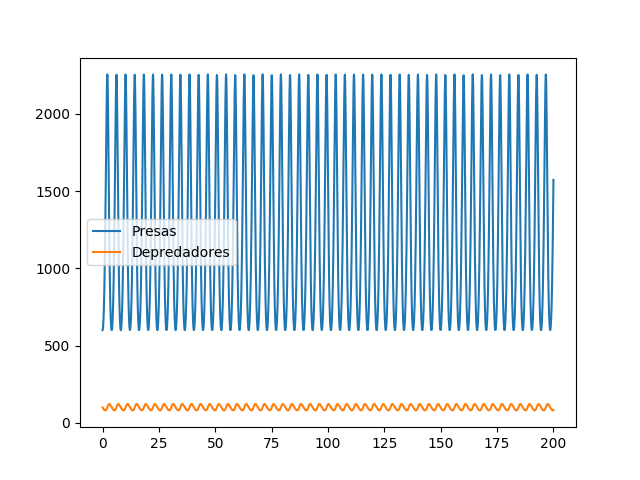
\includegraphics[scale=0.45]{img/a22}
	\subcaption{Evolución de las dos poblaciones en conjunto}
\end{subfigure}%
\begin{subfigure}{.5\textwidth}
	\centering
	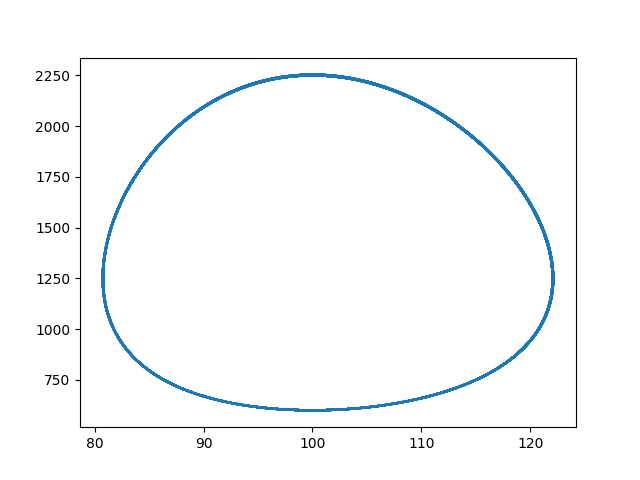
\includegraphics[scale=0.45]{img/circulo-a22}
	\subcaption{Número de presas en función del número de depredadores.}
\end{subfigure}
\caption{Resultados para $a_{22} = 0.3$.}
\label{fig:a22}
\end{figure}

Como podemos comprobar, una mayor tasas de mortalidad implica que la población de depredadores
experimente cambios muy seguidos, creciendo y decreciendo con una frecuencia muy elevada. Estos
crecimientos y decrecimientos afectan también a la población de presas (como es de imaginar), haciendo
que también crezca y decrezca con una frecuencia elevada. Los crecimientos en una de las poblaciones
implican decrecimientos en los de la otra, y viceversa, tal y como pasaba con los ejemplos de la
sección anterior. Podemos ver que esta evolución está en equilibrio, ya que ninguna de las especies llega
al punto en el que se extinga.

De esta sección podemos concluir que no solo es importante conocer los valores iniciales de las
poblaciones, si no que también hay que considerar los valores de los parámetros, ya que estos van
a afectar a las interacciones entre las dos poblaciones de una u otra forma.

\section{Comparativa de los métodos de integración}

Lo último que nos queda por comparar son los métodos de integración utilizados. Por una parte,
tenemos el método de Euler, el cuál es un método simple pero no muy recomendado,
ya que suele tener bastante error de precisión (tiene bastante error de truncatura local).
Por otra parte, tenemos el método de Runge-Kutta, el cuál hemos venido utilizando
hasta ahora. Es bastante más complejo que el de Euler, ya que es de mayor orden,
pero permite obtener mejores resultados en general ya que comete menos error de
precisión.

Para comparar estos métodos, vamos a utilizar distintos intervalos de cálculo. Vamos a
probar los dos métodos con el intervalo de cálculo que llevamos utilizando hasta
ahora, el cuál es $h = 0.1$. También probaremos con valores más pequeños, como
por ejemplo $h = 0.05$ y $h = 0.01$ con el objetivo de ver cuál es el efecto del
intervalo de cálculo en los resultados obtenidos. En cuanto al resto de parámetros, vamos
a utilizar de nuevo 600 presas y 100 depredadores, y el resto de parámetros los dejaremos
tal y como estaban al principio. Los resultados se pueden ver a continuación:

\begin{figure}[H]
\centering
\begin{subfigure}{.5\textwidth}
	\centering
	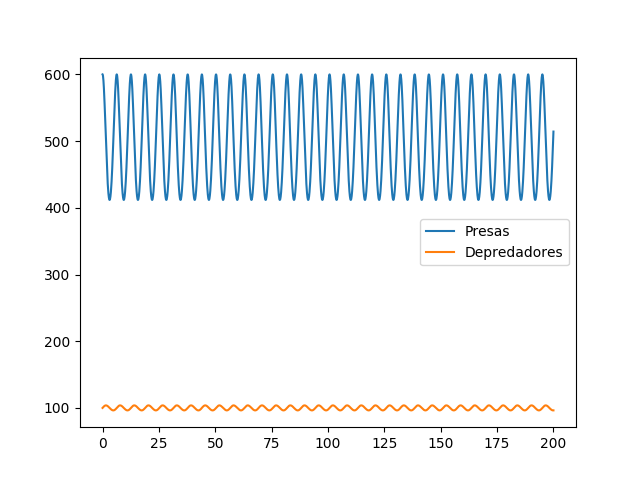
\includegraphics[scale=0.45]{img/rk-0-1}
	\subcaption{Método de Runge-Kutta.}
\end{subfigure}%
\begin{subfigure}{.5\textwidth}
	\centering
	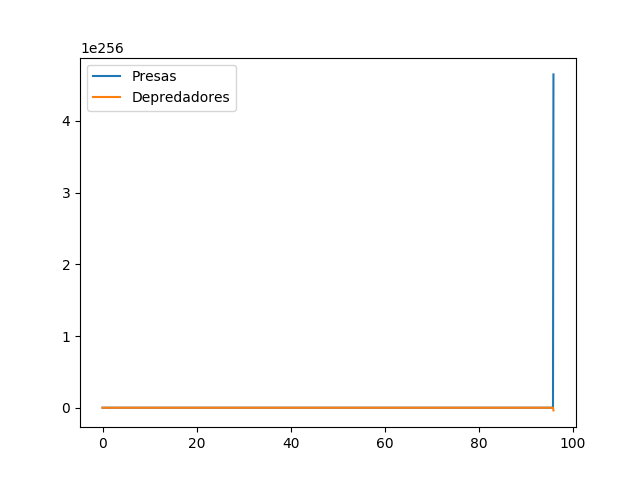
\includegraphics[scale=0.45]{img/eu-0-1}
	\subcaption{Método de Euler.}
\end{subfigure}
\caption{Resultados para $h=0.1$.}
\label{fig:h-0.1}
\end{figure}

\begin{figure}[H]
\centering
\begin{subfigure}{.5\textwidth}
	\centering
	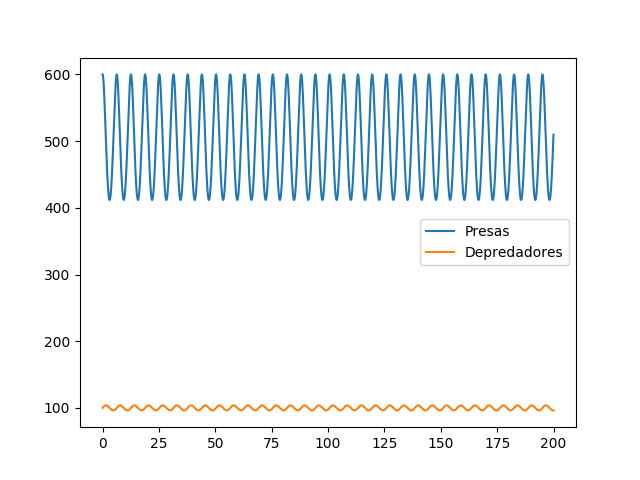
\includegraphics[scale=0.45]{img/rk-0-05}
	\subcaption{Método de Runge-Kutta.}
\end{subfigure}%
\begin{subfigure}{.5\textwidth}
	\centering
	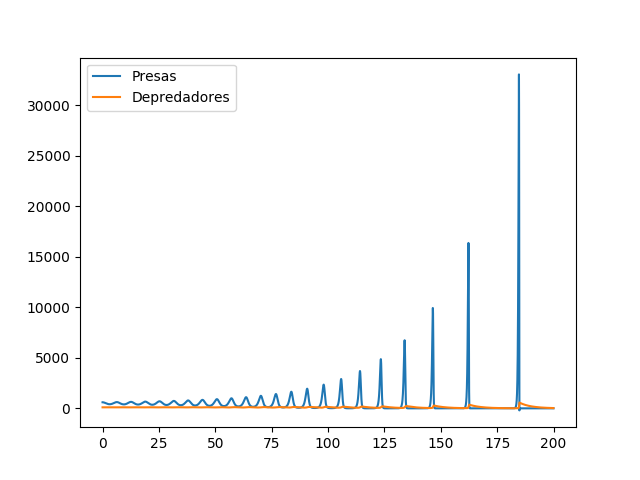
\includegraphics[scale=0.45]{img/eu-0-05}
	\subcaption{Método de Euler.}
\end{subfigure}
\caption{Resultados para $h=0.05$.}
\label{fig:h-0.05}
\end{figure}

\begin{figure}[H]
\centering
\begin{subfigure}{.5\textwidth}
	\centering
	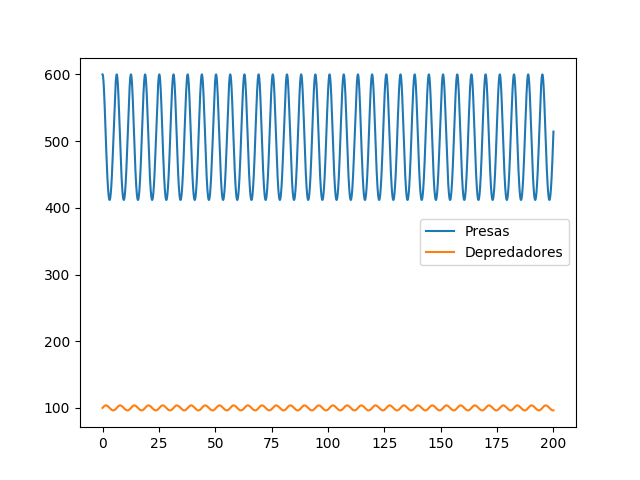
\includegraphics[scale=0.45]{img/rk-0-01}
	\subcaption{Método de Runge-Kutta.}
\end{subfigure}%
\begin{subfigure}{.5\textwidth}
	\centering
	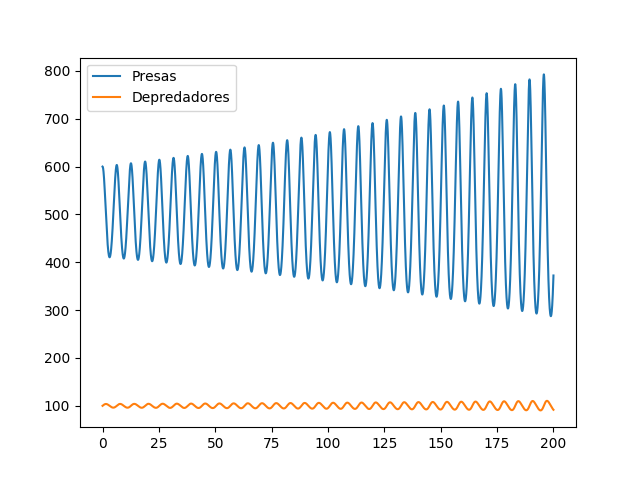
\includegraphics[scale=0.45]{img/eu-0-01}
	\subcaption{Método de Euler.}
\end{subfigure}
\caption{Resultados para $h=0.01$.}
\label{fig:h-0.01}
\end{figure}


En general, podemos ver que los resultados obtenidos para el método de Runge-Kutta
no varían mucho, por no decir casi nada, ya que al ser un método de cuarto orden, permite
obtener unos resultados muy buenos con un error muy bajo. En cambio, si comparamos
el método de Euler con el de Runge-Kutta, vemos que los resultados obtenidos por
el método de Euler son bastante malos en general. Como se puede
observar en la figura \ref{fig:h-0.1}, el método de Euler no es capaz de obtener ningún
tipo de resultado, ya que al ser el intervalo de cálculo tan grande, el error de truncatura
cometido es cada vez más grande, debido a que se va acumulando con el error que ya se tenía
anteriormente, de forma que los resultados que se obtengan sean sin sentido o erróneos.

Al reducir el intervalo de cálculo, como por ejemplo se puede ver en la comparativa de la
figura \ref{fig:h-0.05}, los resultados para el método de Euler siguen siendo malos,
y que se quedan muy lejos de los obtenidos por Runge-Kutta para el mismo intervalo de cálculo.
Si seguimos reduciendo el intervalo de cálculo, vemos que los resultados se van pareciendo
a los obtenidos por Runge-Kutta, aunque solo al principio, ya que luego comienzan a salirse
del rango.

Si para el método de Euler seguimos bajando el valor de $h$, obtenemos los siguientes
resultados:

\begin{figure}[H]
\centering
\begin{subfigure}{.5\textwidth}
	\centering
	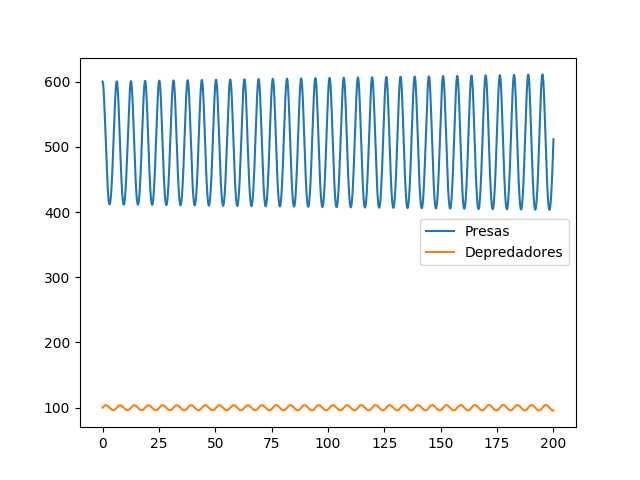
\includegraphics[scale=0.45]{img/eu-0-001}
	\subcaption{Método de Euler con $h=0.001$.}
	\label{fig:eu-0.001}
\end{subfigure}%
\begin{subfigure}{.5\textwidth}
	\centering
	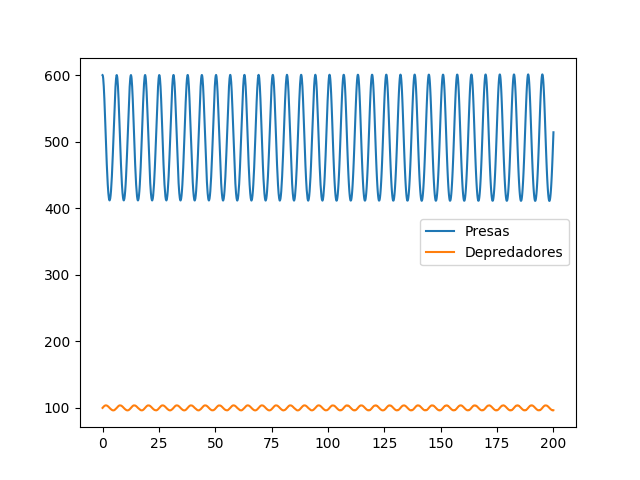
\includegraphics[scale=0.45]{img/eu-0-0001}
	\subcaption{Método de Euler con $h=0.0001$}
	\label{fig:eu-0.0001}
\end{subfigure}
\caption{Método de Euler con valores de $h$ más pequeños.}
\end{figure}

Vemos que en el caso de la figura \ref{fig:eu-0.001} los resultados ya se asemejan más
a los obtenidos por el método de Runge-Kutta, aunque se sigue dando que en las últimas
épocas los resultados empiecen a incrementarse ligeramente. En cambio, para el caso
que se puede observar en la figura \ref{fig:eu-0.0001}, vemos que ahora los resultados
obtenidos por Euler sí que se parecen a los de Runge-Kutta. Sin embargo, para obtener
dichos resultados hemos tenido que reducir mucho el intervalo de cálculo, hasta un
valor de $h = 0.0001$, lo cuál ha resultado en una ejecución más lenta debido
a que el número de cálculos a realizar se ha visto incrementando significativamente.

Por tanto, de aquí podemos concluir que el método de Runge-Kutta, a pesar de ser algo
más complejo, es capaz de ofrecer mejores resultados que el de Euler, que es más sencillo.
Para obtener unos resultados similares al método de Runge-Kutta con Euler, tenemos que
hacer que el intervalo de cálculo sea pequeño a costa de un mayor tiempo de cómputo,
lo cuál puede suponer un problema si no se dispone del hardware adecuado. Por tanto,
tenemos que elegir el método de integración con cuidado, ya que los resultados para
un mismo intervalo de cálculo pueden variar mucho dependiendo de cuál utilicemos.



\end{document}

